% !TeX root = mos-en.tex

%%%%%%%%%%%%%%%%%%%%%%%%%%%%%%%%%%%%%%%%%%%%%%%%%%%%%%%%%%%%%

\begin{center}
\textbf{\LARGE Problems and solutions}
\end{center}

\addcontentsline{toc}{section}{\large Problems and solutions}

\begin{prob}{The sock drawer}
A drawer contains red and black socks. If two socks are drawn at random without replacement the probability that both are red is $\frac{1}{2}$. 

\que{1} How small can the number of black socks in the drawer be? What is the corresponding number of red socks?

\que{2} How small can the number of black socks in the drawer be if the number of black socks is \emph{even}? What is the corresponding number of red socks?
\end{prob}

\solution{1}

\ans{1} Let $r$ be the number of red socks in the drawer and let $b$ the number of black socks.  $r\geq 2$ since two red socks are drawn and $b\geq 1$ since otherwise the probability of drawing two red socks would be $1$.

Multiplying the probabilities for the two draws gives:
\begin{equation}\label{eq.1-a}
P(\textsf{two red})=\frac{r}{r+b} \cdot \frac{(r-1)}{(r-1)+b} = \frac{1}{2}\,.
\end{equation}
Simplifying results in a quadratic equation in the variable $r$:
\begin{equation}\label{eq.quad-for-r}
r^2-r(2b+1)-(b^2-b)=0\,.
\end{equation}
Since $r,b$ are positive integers the discriminant must be the square of an integer:
\begin{equation}\label{eq.discriminant}
(2b+1)^2+4(b^2-b)=8b^2+1
\end{equation}
The discriminant is a square when $b=1$ (its smallest value). From Equation~\ref{eq.quad-for-r}, $r=3$ where we reject the solution $r=0$ because $r\geq 2$. The total number of socks is $4$.

Check: $\frac{3}{4}\cdot\frac{2}{3}=\frac{1}{2}$.

\medskip

\ans{2}
Check positive even values of $b$ to find the smallest one for which the discriminant is a square:
\begin{displaymath}
\renewcommand{\arraystretch}{1}
\begin{array}{r|r|r}
b&8b^2+1&\sqrt{8b^2+1}\\
\hline
2&33&5.74\\
4&129&11.36\\
\mathbf{6}&\mathbf{289}&\mathbf{17}
\end{array}
\end{displaymath}
For $b=6$ the corresponding value for $r$ is $15$.

Check: $\frac{15}{21}\cdot\frac{14}{20}=\frac{1}{2}$.

\solution{2}

\ans{1}
Is the following inequality is true?
\begin{equation}\label{eq.1-b}
\frac{r}{r+b} \stackrel{?}{>} \frac{r-1}{(r-1)+b}\,.
\end{equation}
$r\geq 2, b\geq 1$, so both denominators are positive and we can multiply the two sides:
\begin{eqn}
r(r-1+b)&\stackrel{?}{>}&(r-1)(r+b)\\
r^2-r+rb&\stackrel{?}{>}&r^2-r+rb-b\\
b&\stackrel{?}{>}&0\,.
\end{eqn}
$b>1$ so Equation~\ref{eq.1-b} is true.

By Equations~\ref{eq.1-a}, \ref{eq.1-b}:
\begin{equation}\label{eq.1-c}
\left(\frac{r}{r+b}\right)^2 = \frac{r}{r+b} \cdot\frac{r}{r+b} > \frac{r}{r+b} \cdot \frac{r-1}{(r-1)+b} = \frac{1}{2}\,,
\end{equation}
and similarly:
\begin{equation}\label{eq.1-d}
\left(\frac{r-1}{(r-1)+b}\right)^2  = \frac{r-1}{(r-1)+b}\cdot \frac{r-1}{(r-1)+b}<  \frac{r}{r+b} \cdot \frac{r-1}{(r-1)+b} = \frac{1}{2}\,.
\end{equation}
$r+b$ is non-zero so we can take the square root of Equation~\ref{eq.1-c} and simplify:
\begin{eqn}
\frac{r}{r+b}  &>& \sqrt{\frac{1}{2}}\\
r&>&\frac{b}{\sqrt{2}-1}=\frac{b}{\sqrt{2}-1}\cdot\frac{\sqrt{2}+1}{\sqrt{2}+1}\\
r&>&b(\sqrt{2}+1)\,.
\end{eqn}
Similarly for Equation~\ref{eq.1-d}:
\begin{eqn}
\frac{r-1}{(r-1)+b}&<&\sqrt{\frac{1}{2}}\\
r-1 &<& \frac{b}{\sqrt{2}-1}\\
r-1&<&b(\sqrt{2}+1)\,.
\end{eqn}
Combining both equations we get:
\begin{equation}\label{eq.inequalities}
r-1<(\sqrt{2}+1)b<r\,.
\end{equation}
For $b=1$ we have $2.141 < r< 3.141$ and $b=1,r=3$ is a solution.

\ans{2} Check positive even values of $b$:
\begin{displaymath}	
\renewcommand{\arraystretch}{1}
\begin{array}{r|ccc|c|c}
b& (\sqrt{2}+1)b&<r<& (\sqrt{2}+1)b+1&r&P(\textrm{two reds})\\
\hline
2&4.8&<r<&5.8&5&0.4762\\
4&9.7&<r<&10.7&10&0.4945\\
6&14.5&<r<&15.5&
15&0.5000
\end{array}
\end{displaymath}
Mosteller mentions a connection between this problem and advanced number theory, and gives another solution: $b=35,r=85$.

\medskip
\textbf{Simulation}
\begin{verbatim}
Expectation of both red  = 0.5000
Average of both red for (red =  3, black =  1) = 0.5053
Average of both red for (red = 15, black =  6) = 0.5013
Average of both red for (red = 85, black = 35) = 0.4961
\end{verbatim}

\textbf{Comment}

Neither solution provides a \emph{sufficient} condition for the values of $r,b$. In Solution~1 we derive a necessary condition---by Equation~\ref{eq.discriminant} the discriminant must be an integer---and start searching for values of $b$ that satisfy this requirement. In Solution~2 the necessary condition is that $r,b$ must satisfy the inequalities in Equation~\ref{eq.inequalities} and then we search for values that satisfy the requirement that the probability of two reds must be $0.5$.

I wrote a program to search for solutions. For $r$ near $35$:
\[
\renewcommand{\arraycolsep}{12pt}
\begin{array}{r|r|r|r}
\multicolumn{1}{c|}{r}&
\multicolumn{1}{c|}{b}&
\multicolumn{1}{c|}{\sqrt{8b^2+1}}&
\multicolumn{1}{c}{P(\textsf{two red})} \\\hline
32 & 78  & 90.52 & 0.500917\\
33 & 80  & 93.34 & 0.499368\\
34 & 83  & 96.17 & 0.501474\\
35 & 85  & 99.00 & 0.500000\\
36 & 87  &101.83 & 0.498601\\
37 & 90  &104.66 & 0.500562
\end{array}
\]
Here are the solutions for $b<10^6$:
\[
\begin{array}{r@{\hspace{2em}}r}
\textsf{black} & \textsf{red}\\\hline
1 & 3 \\
6 & 15\\
35 &  85\\
204 &  493\\
1189 &  2871\\
6930 & 16731\\
40391 &  97513\\
235416 & 568345
\end{array}
\]

%%%%%%%%%%%%%%%%%%%%%%%%%%%%%%%%%%%%%%%%%%%%%%%%%%%%%%%%%%%%%

\begin{prob}{Successive wins}
You play a sequence of three games alternately against two players and you win the sequence if you win at least two of the three games \emph{in a row}. The probability that you will win a game against player $P_1$ is $p_1$ and the probability that you will win a game against player $P_2$ is $p_2$. It is given that $p_1>p2$. Which of these sequences gives you a better chance of winning?
\begin{itemize}
\item You play against $P_1,P_2,P_1$ in that order.
\item You play against $P_2,P_1,P_2$ in that order.
\end{itemize}
\end{prob}

\solution{1}

You win if: (a) you win the first two games and lose the last game, (b) you lose the first game and win the last two games, or (c) you win all three games.

Let $p_{121}$ be the probability that you win with the sequence $P_1,P_2,P_1$ and let $p_{212}$ be the probability that you win with the sequence $P_1,P_1,P_2$. Then:
\begin{eqn}
p_{121}&=&p_1p_2(1-p_1) + (1-p_1)p_2p_1 + p_1p_2p_1\\
p_{212}&=&p_2p_1(1-p_2) + (1-p_2)p_1p_2 + p_2p_1p_2\,.
\end{eqn}
You have a better chance of winning with the sequence $P_1,P_2,P_1$ if $p_{121}>p_{212}$, that is, if:
\[
p_1p_2(1-p_1) + (1-p_1)p_2p_1 + p_1p_2p_1 \stackrel{?}{>} 
p_2p_1(1-p_2) + (1-p_2)p_1p_2 + p_2p_1p_2\,.
\]
Cancel $p_1p_2$ from all terms:
\begin{eqn}
(1-p_1)+(1-p_1)+p_1 & \stackrel{?}{>}& (1-p_2)+(1-p_2)+p_2\\
-p_1&\stackrel{?}{>}&-p_2\\
p_2&\stackrel{?}{>}&p_1\,,
\end{eqn}
but by assumption $p_1>p_2$ so you should choose the sequence $P_2,P_1,P_2$,

\solution{2}

The result is counter-intuitive. Intuitively, you should choose to play two games with $P_1$ and one game with $P_2$ because more likely to win games against $P_1$. However, the only way that you can win the sequence is by winning the \emph{middle} game, and, therefore, you should play the middle game against $P_1$, the player you are more likely to defeat.

\textbf{Simulation}
\begin{verbatim}
For p1 = 0.6, p2 = 0.5
Proportion of P121 wins = 0.4166
Proportion of P212 wins = 0.4473

For p1 = 0.6, p2 = 0.4
Proportion of P121 wins = 0.3300
Proportion of P212 wins = 0.3869

For p1 = 0.6, p2 = 0.2
Proportion of P121 wins = 0.1625
Proportion of P212 wins = 0.2141
\end{verbatim}

%%%%%%%%%%%%%%%%%%%%%%%%%%%%%%%%%%%%%%%%%%%%%%%%%%%%%%%%%%%%%

\begin{prob}{The flippant juror}
There are two options to reach a decision: (a) A three-person panel consisting of two members who independently make the correct decision with probability $p$ and one member who makes the correct decision with probability $1/2$. The final decision is determined by a majority vote. (b) A one-person panel whose only member has probability $p$ of making the correct decision. Which option has the higher probability of making the correct decision?
\end{prob}

\solution{}

The three-person panel makes the correct decision if all three members make the correct decision or if any subset of two members makes the correct decision:
\[
P(\textsf{correct decision})=\overbrace{\left(p\cdot p\cdot\frac{1}{2}\right)}^{\textsf{all three correct}}+\;\;\overbrace{\left(p(1-p)\cdot\frac{1}{2}+(1-p)p\cdot\frac{1}{2}+p\cdot p\cdot\frac{1}{2}\right)}^{\textsf{two out of three correct}}=p\,,
\]
so there is no difference between the two options.

\textbf{Simulation}
\begin{verbatim}
Prediction: probabilities of (a) and (b) are equal
For p = 0.25, proportion correct of (a) = 0.5019, (b) = 0.5046
For p = 0.50, proportion correct of (a) = 0.5072, (b) = 0.4970
For p = 0.75, proportion correct of (a) = 0.5062, (b) = 0.5040
\end{verbatim}

%%%%%%%%%%%%%%%%%%%%%%%%%%%%%%%%%%%%%%%%%%%%%%%%%%%%%%%%%%%%%

\begin{prob}{Trials until first success}
\label{p.four}
What is the expectation of the number of throws of a die until a $6$ appears?
\end{prob}

\solution{1}

The probability that the $i$th throw will be the first occurrence of $6$ is the probability of $i-1$ throws of one of the other five numbers times the probability that the $i$th throw will be $6$.

To simplify the notation use $p$ for $1/6$, let $P=P(\textsf{first }\:6\; \textsf{on}\;i \textsf{th throw})$ and let $E=E(\textsf{first throw of}\:6)$: 
\begin{eqnlabels}
\label{eq.first-prob}P&=&(1-p)^{i-1}p\\
\label{eq.first-expec}E&=&1p(1-p)^0 + 2p(1-p)^1+ 3p(1-p)^2+ 4p(1-p)^3 +\cdots =\sum_{i=1}^{\infty} ip(1-p)^{i-1}\,.
\end{eqnlabels}
Without the factor $i$ the sum would be the probability of eventually throwing a $6$:
\begin{equation}\label{eq.geo}
P(\textsf{eventually throwing a}\;6)= \sum_{i=1}^{\infty} p(1-p)^{i-1}=p\cdot\frac{1}{1-(1-p)}=1\,,
\end{equation}
which is not a surprising result.

The calculation of the expectation can be performed as follows:
\[
\renewcommand{\arraycolsep}{2pt}
\begin{array}{lllllllllll}
E&\!\!=\!\!&p(1-p)^0 &+& p(1-p)^1&+& p(1-p)^2&+& p(1-p)^3 &+&\cdots \\
& & &&p(1-p)^1&+& p(1-p)^2&+& p(1-p)^3 &+&\cdots \\
&  &&&& &p(1-p)^2&+& p(1-p)^3 &+&\cdots \\
&&&&&&&&p(1-p)^3 &+&\cdots
\end{array}
\]
The first row is $1$, the sum of the geometric series from Equation~\ref{eq.geo} and the second row is the same infinite geometric series except that the first element is $p(1-p)$ so its sum is:
\[
\frac{p(1-p)}{1-(1-p)}=1-p\,.
\]
Similarly, the sum of the third row will be $(1-p)^2$ and the sum of the $i$th row will be $(1-p)^{i-1}$. Therefore, the expectation is the sum of the infinite geometric series:
\[
E= 1 + (1-p) + (1-p)^2 + (1-p)^3 + \cdots= \frac{1}{1-(1-p)}=\frac{1}{p}=6\,.
\]

\solution{2}

Multiply Equation~\ref{eq.first-expec} by $1-p$ and subtract the result from that equation. The result is the geometric series in Equation~\ref{eq.geo}:
\[
\renewcommand{\arraycolsep}{2pt}
\begin{array}{rclllllllll}
E&=&p(1-p)^0 &+&2p(1-p)^1&+& 3p(1-p)^2&+& 4p(1-p)^3 &+&\cdots\\
E\cdot(1-p)&=&&&p(1-p)^1 &+& 2p(1-p)^2&+& 3p(1-p)^3 &+&\cdots \\
E\cdot(1-(1-p)) &=& p &+& p(1-p)^1 &+& p(1-p)^2 &+& p(1-p)^3 &+&\cdots\\
Ep&=&1\\
E&=&1/p=6\,.
\end{array}
\]

\solution{3}

Consider the first throw separately from the rest of the throws. If the first throw is a $6$ (probability $p$) then one throw is sufficient. Otherwise, if the first throw is not a $6$ (probability $1-p$), then the remaining throws form a sequence identical to the original one so the expectation of this sequence is $E$:
\begin{eqn}
E &=& 1p + (E+1)(1-p)\\
E&=&1/p=6\,.
\end{eqn}

\textbf{Simulation}
\begin{verbatim}
Expectation of first success = 6
Average of first success     = 6.0161
\end{verbatim}

%%%%%%%%%%%%%%%%%%%%%%%%%%%%%%%%%%%%%%%%%%%%%%%%%%%%%%%%%%%%%


\begin{prob}{Coin in a square}

A coin is thrown onto an (unbounded) grid of squares of uniform size. The position of the center of the coin is uniformly distributed within the square in which it lands.

\que{1} Given a square of side $8$ and a coin of radius $3$ what is the probability that the coin lands entirely within the square?

\que{2} For each throw you win $5$ if the coin lands within the square and lose $1$ if it touches a side of the square. What is the expectation of your winnings for each throw?

\que{3} Develop a formula for the probability of the coin landing within the square if the side of the square is $a$ and the radius of the coin is $r<a/4$.
\end{prob}

\solution{}

\ans{1} \ref{f.coins1} shows a square of side $8$ and four circles of radius $3$ inscribed within the corners of the square. The centers of the circles form an inner square of side $2$. Any coin whose center is outside the inner square will touch an edge of the outer square. Since the center of the coin is uniformly distributed, the probability that the coin lands entirely within the square is the ratio of the area of the inner square to the area of the outer square:
\[
P(\textsf{coin lands within the square})=\frac{2\cdot 2}{8\cdot 8} =\frac{1}{16}=0.0625\,.
\]
\begin{figure}[tb]
\begin{center}
\begin{subfigure}{.43\textwidth}
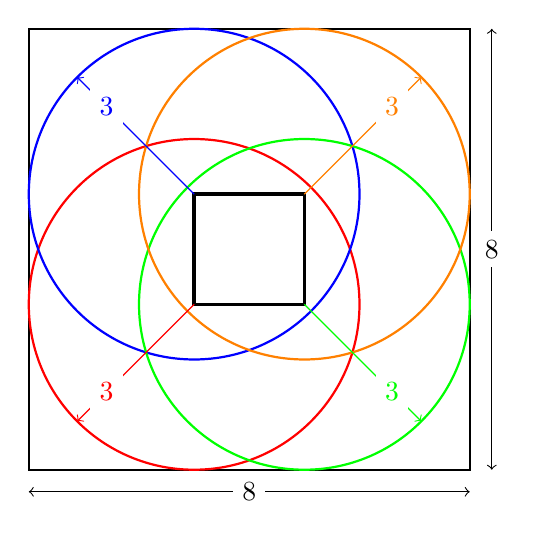
\begin{tikzpicture}[scale=.7]
\coordinate (c1) at (3,3);
\coordinate (c2) at (3,5);
\coordinate (c3) at (5,3);
\coordinate (c4) at (5,5);
\draw[very thick] (c1) -- (c3) -- (c4) -- (c2) -- cycle;
\draw[thick] (0,0) rectangle +(8,8);
\draw[color=red,thick] (c1) circle[radius=3];
\draw[color=blue,thick] (c2) circle[radius=3];
\draw[color=green,thick] (c3) circle[radius=3];
\draw[color=orange,thick] (c4) circle[radius=3];
\vertexcolor{c1}{red};
\vertexcolor{c2}{blue};
\vertexcolor{c3}{green};
\vertexcolor{c4}{orange};
\draw[<->] (0,-.4) -- node[fill=white] {$8$} (8,-.4);
\draw[<->] (8.4,0) -- node[fill=white] {$8$} (8.4,8);
\draw[->,red] (3,3) -- node[near end,fill=white] {$3$} +(-135:3);
\draw[->,blue] (3,5) -- node[near end,fill=white] {$3$} +(135:3);
\draw[->,green] (5,3) -- node[near end,fill=white] {$3$} +(-45:3);
\draw[->,orange] (5,5) -- node[near end,fill=white] {$3$} +(45:3);
\end{tikzpicture}
\caption{Coins contained in the square}\label{f.coins1}
\end{subfigure}
\hspace{3em}
\begin{subfigure}[b]{.43\textwidth}
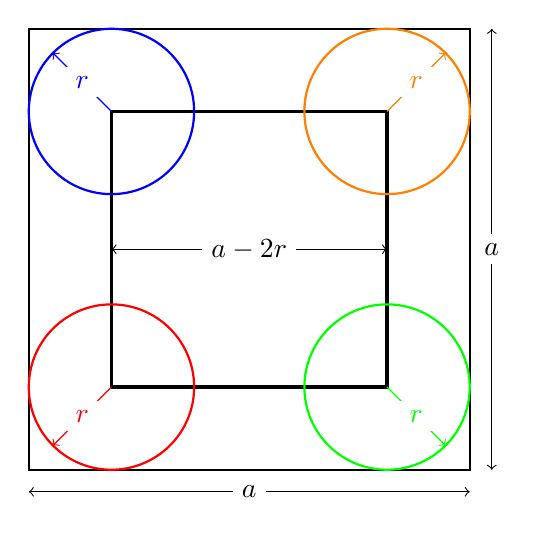
\begin{tikzpicture}[scale=.7]
\coordinate (c1) at (1.5,1.5);
\coordinate (c2) at (1.5,6.5);
\coordinate (c3) at (6.5,1.5);
\coordinate (c4) at (6.5,6.5);
\draw[very thick] (c1) -- (c3) -- (c4) -- (c2) -- cycle;
\draw[thick] (0,0) rectangle +(8,8);
\draw[color=red,thick] (c1) circle[radius=1.5];
\draw[color=blue,thick] (c2) circle[radius=1.5];
\draw[color=green,thick] (c3) circle[radius=1.5];
\draw[color=orange,thick] (c4) circle[radius=1.5];
\vertexcolor{c1}{red};
\vertexcolor{c2}{blue};
\vertexcolor{c3}{green};
\vertexcolor{c4}{orange};
\draw[<->] (0,-.4) -- node[fill=white] {$a$} (8,-.4);
\draw[<->] (8.4,0) -- node[fill=white] {$a$} (8.4,8);
\draw[->,red] (1.5,1.5) -- node[fill=white] {$r$} +(-135:1.5);
\draw[->,blue] (1.5,6.5) -- node[fill=white] {$r$} +(135:1.5);
\draw[->,green] (6.5,1.5) -- node[fill=white] {$r$} +(-45:1.5);
\draw[->,orange] (6.5,6.5) -- node[fill=white] {$r$} +(45:1.5);
\draw[<->] (1.5,4) -- node[fill=white] {$a-2r$} (6.5,4);
\end{tikzpicture}
\caption{Coins in a large square}\label{f.coins2}
\end{subfigure}
\end{center}
\end{figure}

\ans{2}
\[
E(\textsf{winnings per throw})=5\cdot\frac{1}{16}\,+\,(-1)\cdot\frac{15}{16}=-\frac{10}{16}=-0.625\,.
\]

\ans{3} Figure~\ref{f.coins2} shows four circles inscribed in the corners of the square. The side of the inner square is $a-2r$ so:
\[
P(\textsf{coin lands within the square})=\frac{(a-2r)^2}{a^2}\,.
\]
\textbf{Simulation}
\begin{verbatim}
For side = 8, radius = 1:
Probability of landing within the square = 0.5625
Proportion landing within the square     = 0.5704
For side = 8, radius = 2:
Probability of landing within the square = 0.2500
Proportion landing within the square     = 0.2481
For side = 8, radius = 3:
Probability of landing within the square = 0.0625
Proportion landing within the square     = 0.0639
For side = 8, radius = 4:
Probability of landing within the square = 0.0000
Proportion landing within the square     = 0.0000
\end{verbatim}

%%%%%%%%%%%%%%%%%%%%%%%%%%%%%%%%%%%%%%%%%%%%%%%%%%%%%%%%%%%%%

\begin{prob}{Chuck-a-luck}
Choose number $n$ between $1$ and $6$ and throw three dice. If $n$ does not appear on any of the dice you lose $1$; if $n$ appears on one die you win $1$; if $n$ appears on two dice you win $2$; if $n$ appears on three dice you win $3$. What is the expectation of your winnings?
\end{prob}

\solution{}

Let $P(k)$ be the probability that $n$ appears on $k$ dice. Then:
\[
E(\textsf{winnings per throw})=-1 P(0) + 1 P(1) + 2 P(2) + 3 P(3)\,.
\]
The throws of the three dice are independent so:
\begin{eqn}
E(\textsf{winnings per throw}) &=& 
-1 \dischoose{3}{0}\left(\frac{1}{6}\right)^0\left(\frac{5}{6}\right)^3
+1\dischoose{3}{1}\left(\frac{1}{6}\right)^1\left(\frac{5}{6}\right)^2+\\
&&\;\;\; 2{3\choose 2}\left(\frac{1}{6}\right)^2\left(\frac{5}{6}\right)^1+
3\dischoose{3}{3}\left(\frac{1}{6}\right)^3\left(\frac{5}{6}\right)^0\\
&=& \frac{1}{216}(-125+75+30+3)\approx -0.0787\,.
\end{eqn}

\textbf{Simulation}
\begin{verbatim}
Expectation of winnings = -0.0787
Average winnings        = -0.0724
\end{verbatim}

%%%%%%%%%%%%%%%%%%%%%%%%%%%%%%%%%%%%%%%%%%%%%%%%%%%%%%%%%%%%%

\begin{prob}{Curing the compulsive gambler}
Roulette is a game played with a wheel having $38$ numbered pockets: $18$ red, $18$ black and $2$ green.\footnote{There are two green pockets in American roulette and one green pocket in European roulette.} The wheel is spun and a ball lands in a random pocket with a uniform distribution. You select one of the red or black pockets and bet $1$ that the ball will land in that pocket. If so you receive $36$. Your net winnings are actually $35$ because the the $36$ includes the $1$ bet which is returned.

\que{1} What is the expectation your winnings if you play $36$ round of roulette?

\que{2} Your friend offers to bet you $20$ that after $36$ rounds you will have \emph{lost} money. What is the expectation of your winnings, taking into account the money won or lost from both the game and the bet with your friend?
\end{prob}

\solution{}

\ans{1} The probability of winning a single round is $1/38$ so:
\begin{eqn}
E(\textsf{winnings in one round})&=&35\cdot \frac{1}{38} + (-1)\cdot\frac{37}{38} = -\frac{2}{38} \approx -0.0526\\
E(\textsf{winnings in}\;36\;\textsf{rounds})&=&36\cdot -0.05266=-1.8947\,.
\end{eqn}

\ans{2}
Consider the four outcomes of playing roulette for $36$ rounds:
\begin{itemize}
\item If you lose all the rounds you lose $36$.
\item If you win one round you win $35$ and you lose $35$ on the other rounds no money is won or lost.
\item If you win two rounds you win $70$ and you lose $34$ on the other rounds for a net win of $36$.
\item In general if you win $k$ rounds for $2<k\leq 36$ your net win is $35k - (36-k)>0$.
\end{itemize}
Therefore, you lose the bet only if you lose all rounds:
\begin{eqn}
P(\textrm{losing\ } 36 \textrm{\ rounds})&=&\left(\frac{37}{38}\right)^{36}\approx 0.3829\\
E(\textsf{total winnings})&=&\overbrace{-1.8947}^{\textsf{\small E of all rounds}}+\;\;
\overbrace{-20\cdot 0.3829}^{\textsf{\small lose bet}} \;+\; \overbrace{20\cdot (1-0.3829))}^{\textsf{\small win bet}} \approx 2.7904\,.
\end{eqn}
Clearly you should take the bet!

\textbf{Simulation}
\begin{verbatim}
Expectation of winning a round = -0.0526
Average winnings for a round   = -0.0593
\end{verbatim}
The simulation showed a large variance which was reduced by running one million trials.

%%%%%%%%%%%%%%%%%%%%%%%%%%%%%%%%%%%%%%%%%%%%%%%%%%%%%%%%%%%%%

\begin{prob}{Perfect bridge hand}
Randomly select $13$ cards from a deck. What is the probability that they will all be of the same suit?
\end{prob}

\solution{1}

There are $\dischoose{52}{13}$ ways of selecting $13$ cards from a deck of $52$ cards. Only four of them consist of $13$ cards from the same suit:
\[
P(\textsf{selecting}\;13\;\textsf{of same suit})=\frac{4}{\dischoose{52}{13}}=\frac{4\cdot 13!\cdot 39!}{52!}\approx 6.2991\times 10^{-12}\,.
\]

\solution{2}

There are $52$ ways of selecting the first card, then $12$ ways of selecting the second card of the same suit from the remaining $51$ cards, $11$ ways of selecting a third card, and so on:
\[
P(\textsf{selecting}\;13\;\textsf{cards of the same suit})=\frac{52}{52}\cdot \frac{12}{51}\cdot \frac{11}{50} \cdots  \frac{1}{40}= \frac{12!}{51!/39!}\approx 6.2991\times 10^{-12}\,.
\]

\textbf{Simulation}
There is no point in running a simulation with $52$ cards because the result would almost certainly be zero. A simulation was run with a deck of $16$ cards and $4$ suits.

\begin{verbatim}
Probability of perfect hand = 0.0022
Proportion perfect hand     = 0.0020
\end{verbatim}

%%%%%%%%%%%%%%%%%%%%%%%%%%%%%%%%%%%%%%%%%%%%%%%%%%%%%%%%%%%%%

\begin{prob}{Craps\annotate{D}}
Craps is a played with a pair of dice. On the first throw you win if the sum of the numbers is $7$ or $11$ and you lose if the sum is $2$, $3$ or $12$. If the sum on the first throw is $n=4,5,6,8,9,10$ (called a \emph{point}), continue to throw the dice until the sum is the point $n$ (a win) or $7$ (a loss).

\que{1} What are the probabilities of the events on the first throw: winning, losing, neither?

\que{2} What is the probability of a win?
\end{prob}

\solution{1}

\ans{1} The probability of any outcome in a throw of a die is uniformly distributed and is equal to $1/6$. Since the outcomes of a throw of a pair of dice are independent, the probability of any outcome is $1/36$. The number of ways of obtaining each of the events---the sum of a pair of dice is equal to one of the points $2,\ldots,12$---is:
\[
\begin{array}{l|rrrrrrrrrrr}
\textrm{Sum} & 2 & 3 & 4 & 5 & 6 & 7 & 8 & 9 & 10 & 11 & 12\\\hline
\textrm{Pairs} & 1 & 2 & 3 & 4 & 5 & 6 & 5 & 4 & 3 & 2 & 1
\end{array}
\]
On the first throw there are $8$ ways of throwing $7$ or $11$ so the probability of winning is $8/36$ and there are $4$ ways of throwing $2,3,12$ so the probability losing is $4/36$. The probability of neither winning nor losing on the first throw is:
\[
1 - \frac{8}{36} - \frac{4}{36} = \frac{24}{36}\,.
\]

\ans{2}
Consider two cases:
\begin{itemize}
\item The point is $4$. The probability of winning on the second throw (a $4$) is $3/36$ and the probability of losing (a $7$) is $6/36$. The probability of neither winning nor losing is $1-(3/36)-(6/36)=27/36$.
\item The point is $8$. The probability of winning on the second throw (an $8$) is $5/36$ and the probability of losing (a $7$) is $6/36$. The probability of neither winning nor losing is $1-(5/36)-(6/36)=25/36$.
\end{itemize}
We see that the probability of winning must be computed separately for each of the points $4,5,6,8,9,10$, so we develop a general formula for the probability.

Let $P_n$ be the probability of winning by throwing the point $n$ on a throw and let $Q_n$ the probability of neither winning nor losing on a throw is the point is $n$. $W_n$, the probability of winning by \emph{eventually} throwing the point $n$ after the first throw, is computed by adding:
\begin{itemize}
\item The probability of throwing the point on the second throw.
\item The probability of neither winning nor losing on the second throw and throwing the point on the third throw.
\item The probability of neither winning nor losing on the second and third throws and throwing the point on the fourth throw,
\end{itemize}
and so on:
\begin{eqn}
W_n&=&P_n + Q_n P_n + Q_n^2 P_n+ Q_n^3 P_n  + \cdots\\
&=&P_n\left(1+Q_n^1 + Q_n^2+ Q_n^3  + \cdots\right)\\
&=&P_n\left(\frac{1}{1-Q_n}\right)\,.
\end{eqn}
You lose the game on any throw after the first if you throw a $7$ with probability $6/36$ so:
\begin{eqn}
Q_n &=& 1-P_n-(6/36)\\
W_n&=&\frac{P_n}{P_n+(6/36)}\,.
\end{eqn}
$W_n$ for the six points are:
\[
\renewcommand{\arraystretch}{2}
\begin{array}{lcccccc}
n   & 4 & 5 & 6 & 8 & 9 & 10 \\\hline
P_n & \disfrac{3}{36} & \disfrac{4}{36} & \disfrac{5}{36} & \disfrac{5}{36} & \disfrac{4}{36} & \disfrac{3}{36} \\
%1-Q_n & \disfrac{9}{36} & \disfrac{10}{36} & \disfrac{11}{36} & \disfrac{11}{36} & \disfrac{10}{36} & \disfrac{9}{36} \\
W_n & \disfrac{3}{9} & \disfrac{4}{10} & \disfrac{5}{11} & \disfrac{5}{11} & \disfrac{4}{10} & \disfrac{3}{9}
\end{array}
\]
$W$, the probability of winning, can be computed by adding the probability of winning on the first throw to the sum of the probabilities for the six wins on points each multiplied by the probability of throwing \emph{that point} on the first throw:
\begin{equation}\label{eq.9-a}
W=\frac{8}{36}+\sum_{n\in\{4,5,6,8,9,10\}} P_nW_n \approx 0.4929\,.
\end{equation}
The casino's probability of winning a single game of craps is
only $0.5-0.4929\approx 0.5\%$ but the law of large numbers ensures that they will eventually win and you will eventually lose!

\solution{2}

\ans{2} Consider the following sequences of throws where the point is $4$:
\[
\begin{array}{rrrrrrrrrrr}
4 & 8 & 9 & 9 & 9 & 8 & 8 & 8 & 9 & 8 & 4\\
4 & 8 & 9 & 9 & 9 & 8 & 8 & 8 & 9 & 8 & 7\\
4 & 9 & 9 & 9 & 8 & 8 & 4
\end{array}
\]
The games only terminates if a $4$ is thrown (win) or a $7$ is thrown (loss), so an appearance of an $8$ or a $9$ doesn't affect the result. Therefore, once a point has been thrown, the probability of winning is the conditional probability that a $4$ is thrown given that a $4$ or  a $7$ is thrown. Let $f$ be the event that a $4$ is thrown and $s$ be the event that a $7$ is thrown. Then:
\[
P(f|f\cup s) = \disfrac{P(f)\cap P(f\cup s)}{P(f\cup s)}=\disfrac{P(f)}{P(f\cup s)}=\disfrac{3/36}{(3+6)/36}=\disfrac{3}{9}\,,
\]
which is exactly the result $W_4$ in the table above. After computing $W_n$ for all points, Equation~\ref{eq.9-a} can be used to compute $W$.

Conditional probability is implicitly used in the first solution because $W_n$ is a probability that is conditional on the first throw resulting in the point $n$.

\textbf{Simulation}
\begin{verbatim}
Probability of winning = 0.4929
Proportion of wins     = 0.4948
\end{verbatim}

%%%%%%%%%%%%%%%%%%%%%%%%%%%%%%%%%%%%%%%%%%%%%%%%%%%%%%%%%%%%%

\refstepcounter{problem}  % 10. An experiment in personal taste

